\emph{Nota:} Como vamos a hablar mucho de las distintas podas vamos a denominarlas de la siguiente manera:
\begin{itemize}
\item Poda 1: Si aunque ponga piezas en los casilleros que me queda revisar, no llego a alcanzar la cantidad de piezas de la solución óptima encontrada a ese momento, corto.
\item Poda 2: Similar a la poda 1, pero además revisa hasta $m$ casillas para adelante teniendo en cuenta las restricciones ya existentes en el tablero.
\end{itemize}

En este ejercicio, vamos a enfocar la experimentación orientándolo a la comparación entre las distintas podas, así como también comparar las mismas contra no usar ninguna poda. Cabe aclarar que no usar ninguna poda tiene un método de corte \emph{naïf}: cortar si logré llenar el tablero.

En los siguientes gráficos podemos observar que utilizar podas mejora drásticamente el tiempo de ejecución, respecto a no utilizar podas.

\begin{center}
  \begin{figure}[H]
    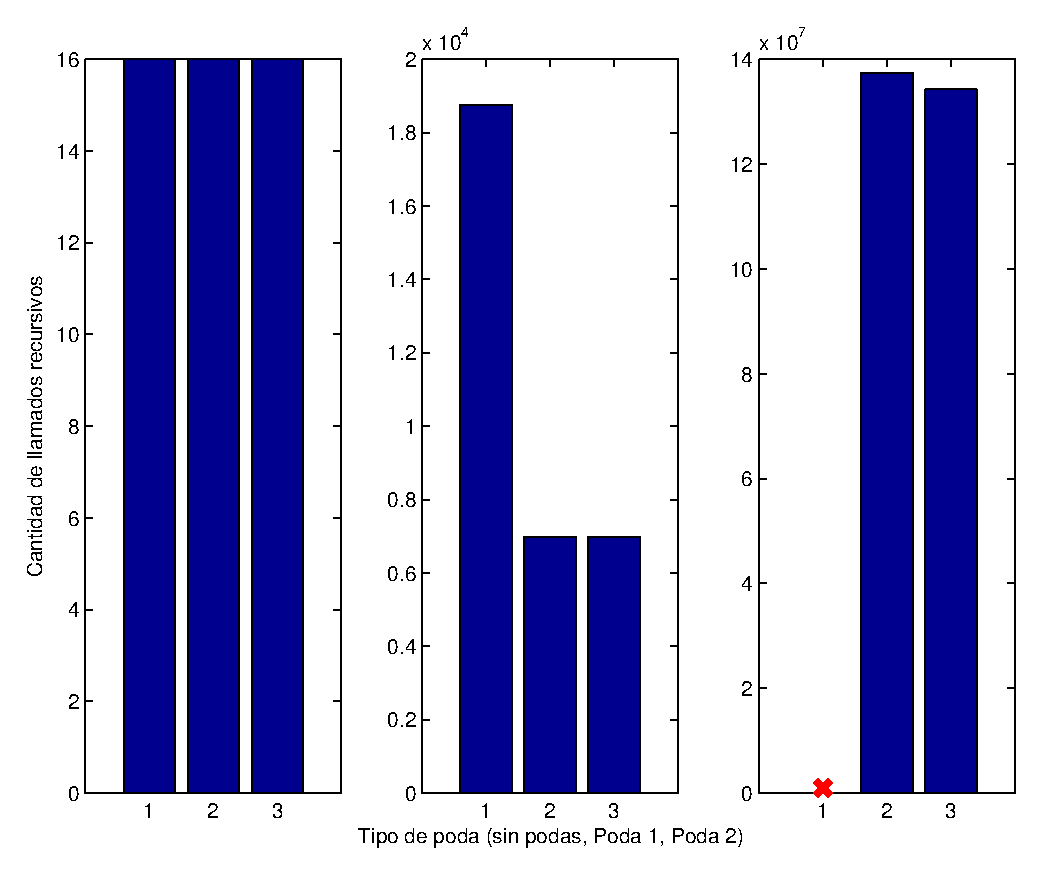
\includegraphics[width=0.5\linewidth]{problema3/graficos/comparacion_podas_todas_instancias_llamados.eps}
    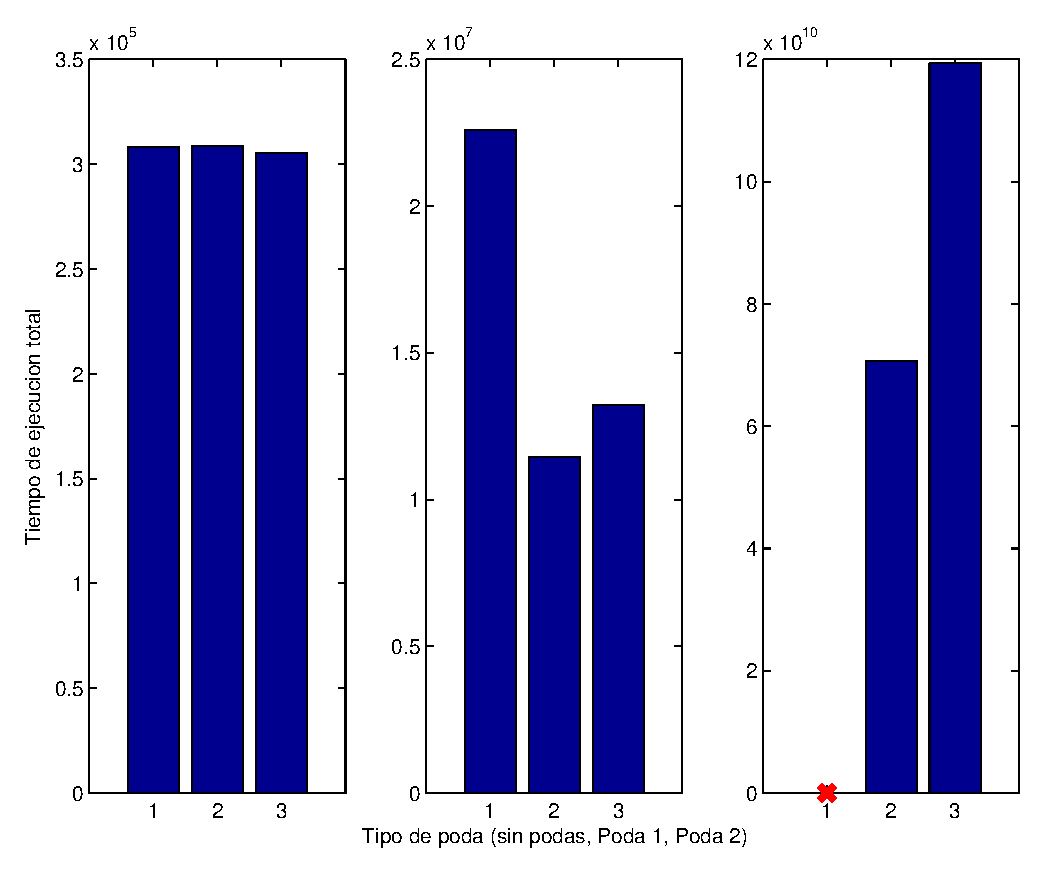
\includegraphics[width=0.5\linewidth]{problema3/graficos/comparacion_podas_todas_instancias_tiempo.eps}
    \caption{Comparación con y sin podas. Izquierda: llamados recursivos, Derecha: tiempo}
    \label{fig:problema3-sin-y-con-podas}
  \end{figure}
\end{center}

En estos gráficos podemos observar que utilizar podas mejora tanto en la cantidad de llamados recursivos, así como también mejora en tiempo de ejecución. A su vez, si bien la cantidad de llamados recursivos que realiza el algoritmo al utilizar la poda 2 es menor a la cantidad de llamados recursivos que realiza al utilizar la poda 1, el tiempo de ejecución del algoritmo utilizando poda 2 es claramente mayor a utilizar la poda 1. Esto nos lleva a pensar que para casos chicos, es mejor utilizar la poda 1 ya que el tiempo de ejecución es menor.

Una de las razones que no usar podas es tan malo es que revisa todos los tableros posibles, y recién una vez revisados todos termina (salvando el caso en que justo encuentre el tablero completo). Esto implica que ya para tableros de 3*3 es un número grande de tableros posibles, y para tableros aún más grandes el algoritmo tarda una cantidad incomparable de tiempo con respecto a las podas. Por esta razón, sin podas no esta presente en el tercer gráfico de arriba, ni en los gráficos de abajo.

Los siguientes 50 casos sólo van a ser comparados utilizando podas.

\begin{center}
  \begin{figure}[H]
    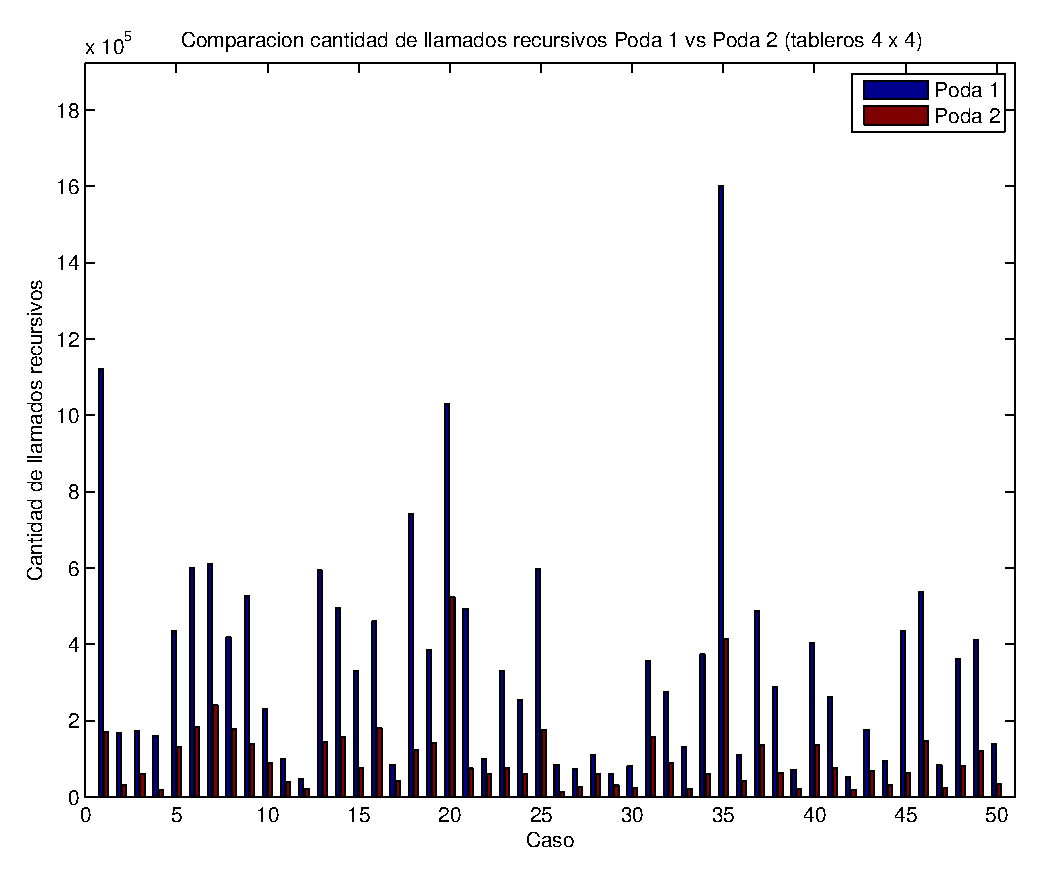
\includegraphics[width=\linewidth]{problema3/graficos/comparacion_podas1y2_llamados_recursivos.eps}
    \caption{Comparación de podas, según llamados recursivos}
    \label{fig:problema3-podas-llamados}
  \end{figure}
\end{center}

\begin{center}
  \begin{figure}[H]
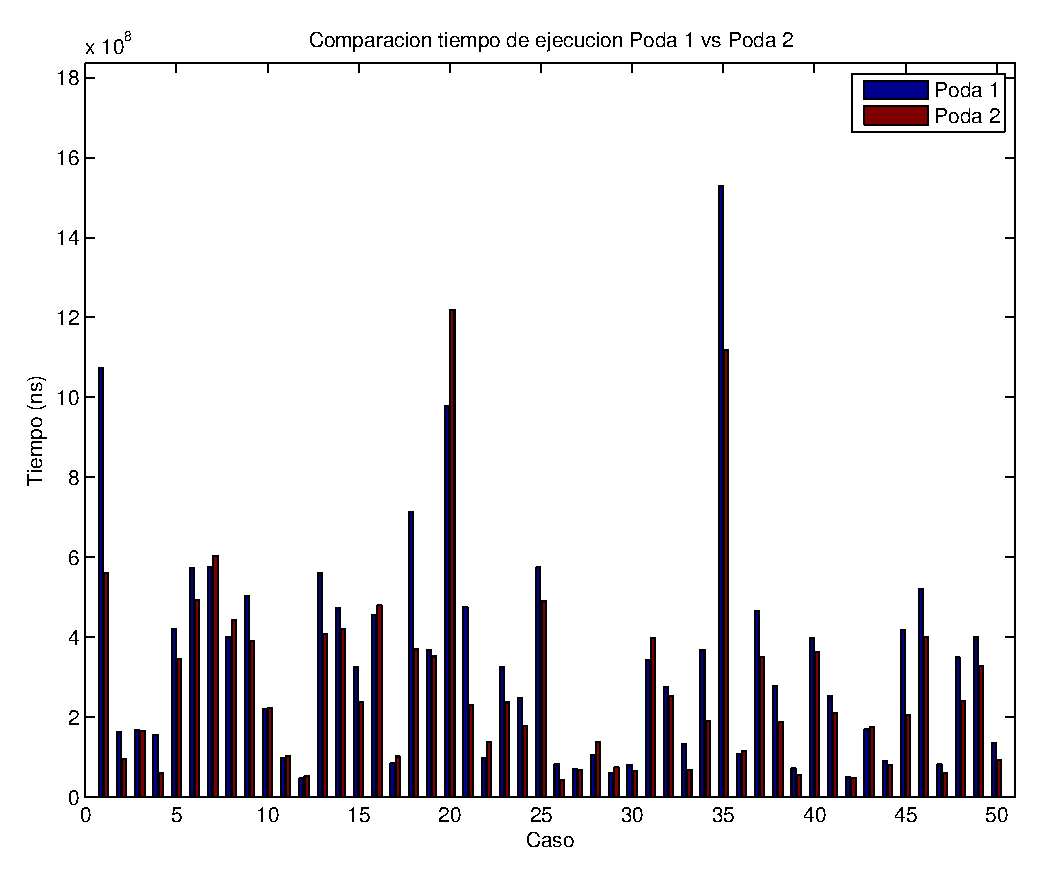
\includegraphics[width=\linewidth]{problema3/graficos/comparacion_podas1y2_tiempo.eps}
    \caption{Comparación de podas, según tiempo de ejecución}
    \label{fig:problema3-podas-tiempo}
  \end{figure}
\end{center}


En el gráfico \ref{fig:problema3-podas-llamados}, podemos observar claramente que la poda 2 logra podar mas casos y por consiguiente, realiza menos llamados recursivos. Sin embargo, en la figura \ref{fig:problema3-podas-tiempo} podemos observar que no siempre logra compensar lo suficiente el costo adicional de $O(m)$ para lograr que sea considerablemente mejor.

Como ejemplo, el caso 35 logra podar lo suficiente para lograr 4 veces menos llamados recursivos. Sin embargo, logra solamente ser un 25\% (aproximadamente) mejor en tiempo de ejecución.

Por otro lado, la poda 1 también tiene beneficios. Es considerablemente más fácil de implementar que la poda 2. A su vez, la poda 1 no depende de la cantidad de colores existentes, mientras que la poda 2 sí lo hace. La poda 2 crea un $vector<int>$ donde la cantidad de posiciones se corresponde con la cantidad de colores existentes. Si bien no es un problema muy grave, puede ocurrir que sí lo sea si tenemos una computadora con memoria acotada y tenemos un caso donde la cantidad de colores es muy alta, como por ejemplo un millón de colores.

Curiosamente, si bien utilizar la poda 1 incurre en una menor cantidad de tiempo de ejecución para casos mas chicos (como por ejemplo tableros de tamaño de 3*3), esto no se mantiene para casos más grandes (como tableros de tamaño 4*4). Es decir, la poda 2 comienza a tener más importancia cuando el tablero es más grande. Creemos que esto se debe a que las podas que realiza la poda 2 tienen más impacto con respecto al costo de realizar dicha poda en tableros de tamaño más grande.